\documentclass[11pt,a4paper]{article}
\usepackage{amsmath,amssymb}
\usepackage{graphicx}
\usepackage{setspace}
\usepackage{tikz}
\usepackage[margin=1in]{geometry}
\usepackage{booktabs}
\usepackage{multirow}
\usepackage[numbers]{natbib}
\usepackage{natbib}
\usepackage{parskip}
\usepackage{tablefootnote}
\usepackage[linesnumbered,ruled,vlined]{algorithm2e}
\newcommand{\citeboth}[1]{\citeauthor{#1} \citep{#1}}


\usepackage[
    colorlinks=true,      % Enable colored links
    linkcolor=green,       % Color for internal links (e.g., \ref, \pageref)
    citecolor=blue,       % Color for citations
    urlcolor=blue,        % Optional: Set PDF metadata
]{hyperref}


\title{Investigating the Impact of Macroeconomic Indicators 
on the FTSE 250 Index Using Machine Learning Methods}
\author{Mateen Khan}
\date{}

\begin{document}

\maketitle

\begin{abstract}
    Investment decisions and economic policy are highly influenced by 
    macroeconomic variables and the stock market. Econometric models
    have been the predominant tools in this context. The aim of this study is to analyse the impacts of some especially important macroeconomic
    indicators on the FTSE250 
    (Financial Times Stock Exchange 250 Index), using monthly data 
    from  October 1993 to April 2024 using an ARDL model, obtaining 
    quantifiable estimates for the long-term and short-term impacts of the variables
    on the FTSE250. The efficacy of Radial Basis Function 
    Neural Networks (RBF-NN) in this problem domain is then investigated. It is established 
    the RBF-NN is a competent short-term forecasting tool, and is able to 
    provide an alternative approach to standard econometric models in measuring the long-term influence of
    macroeconomic variables on the stock market.
\end{abstract}

\section{Introduction}

The stock market has played a central role in the economy and 
political ascent of many states ever since its inception. 
Accordingly, any instabilities that have arisen in the stock market 
throughout history have had far-reaching destabilising effects on the 
economy; the Mississippi Bubble (1717-1720) was an early example of the 
dangers that stock markets carry, where the French colonial administration 
in America went bankrupt as a result of a speculative bubble. With the
growing interconnectedness of markets, the stock market as an institution 
has also contributed significantly to global disasters such as the Great 
Depression and the Global Financial Crisis of 2008/9. Thus, economic 
policymakers and administrators require forecasts for how policy changes or 
unexpected economic trends may impact the economy through the stock market. 

Investors and traders are also intimately affected by the 
fluctuations of economic factors due to their destabilising effect on firms.
The ability to forecast stock index price changes allows 
investors to optimise their trading strategies, enabling them to make
informed decisions about when to buy or sell assets. 
Additionally, in a globalised economy, the interconnectedness of 
markets means that events in one region may have significant effects worldwide, 
making it even more critical for investors to stay ahead of potential market movements.

The traditional methods that have been leveraged in both of these contexts have been econometric.
Machine learning methods, particularly neural networks, have emerged as powerful alternatives capable
of capturing complex relationships in financial data, and thereby providing more
accurate forecasts than econometric models.

In this study, first an Autoregressive Distributed Lag (ARDL) model in conjunction with an Error Correction Model (ECM), is employed to investigate 
the different effects of selected macroeconomic variables on the FTSE250 Index over the January 1993 - March 2024 period.
Second, the efficacy of a Radial Basis Function Neural Network (RBF-NN) is tested in forecasting the price movements of the FTSE250 based on the selected macroeconomic indicators, over the short-term 
(5 months) and long-term (57 months), the former intended to inform investors and the latter to provide
economic policymakers with a tool to measure the influence of macroeconomic variables on the price of the stock market. 


The FTSE250 is utilised as the measure of the UK stock market, because unlike the 
FTSE100 its overseas share of earnings is 
roughly $50\%$, similar to the S\&P 500. In contrast, nearly $80\%$ of the FTSE$100$'s earnings 
are from overseas. This is reflected in the constitution of the respective indices, with 
the FTSE250 historically resembling the structure 
of the UK economy more closely than the FTSE100.

The macroeconomic variables considered are inflation, indicated by the Consumer Price
Index (CPI); interest rate, represented by the Bank of England policy rate; the exchange rate, 
represented by the USD/GBP exchange rate; and the money supply, represented by the 
M3 measure of money supply, preferred over other 
measures of the money supply because it considers more assets than M2 money supply 
but does not include extremely illiquid assets as the M4 measure does. The selection 
of these variables was based on the literature and the structure of the UK economy since 
the establishment of the FTSE250 Index.

The remainder of the paper is organised as follows. 
Section 2 presents a review of the literature in this problem space, and explains the rationale behind our selection of macroeconomic variables.
Section 3 covers the data utilised in the study. Section 4 outlines the ARDL-ECM model, our methodology, and our results describing
the effect of the selected macroeconomic variables on the FTSE250. Section 5 constructs the RBF-NN model, and presents the short-term and long-term
forecasts for the FTSE250 Index price movements, based on our selected macroeconomic variables. Section 6 concludes the study.

\section{Literature Review}

\subsection{Stock Market-Macroeconomy Relationship}

There are a number of works which investigate the impact of 
the selected macroeconomic variables
on the stock market.

\subsubsection{Inflation}

The Fisher hypothesis states that nominal interest rates adjust to expected 
inflation, implying market efficiency as firms correctly anticipate inflation 
and adjust prices. This was tested this in the US stock market by \citeboth{jaffe1976}, and
\citeboth{bodie1976} who both found a negative relationship between inflation and stock returns.
To account for this,
\citeboth{mogdiliani1979} proposed the Inflation Illusion Hypothesis, 
arguing that investors overestimate the discount rate in valuations, leading to mispricing. 
\citeboth{gultekin1983} and \citeboth{firth1979}, however, found that the relationship between nominal stock returns and inflation in the UK is positive, and that real returns on UK stocks have remained stable even as inflation varied.
Later, \citeboth{hasan2008} provided evidence against this, challenging the Fisher hypothesis.

\subsubsection{Interest Rate}

Interest rates, being the cost of borrowing, directly impact firms by increasing financing costs, reducing profitability, and lowering growth prospects. For consumers, higher rates raise borrowing costs, leading to reduced spending and demand, which further lowers corporate profitability. 
The empirical research supports this theory: \citeboth{alam2009} found a significant inverse relationship between interest rates and stock prices across multiple countries from 1988 to 2003; 
\citeboth{talla2013} observed a negative relationship between interest rates and stock prices on the Stockholm Stock Exchange; 
\citeboth{demir2019} reported similar findings for the Turkish Stock Exchange. In the case of the UK, \citeboth{neifar2023} used a Non-Linear ARDL model to find a significantly negative long-run relationship between interest rates and the UK stock market. Higher interest rates also encourage a shift from stocks to safer 
assets like bonds, this is known as the flight-to-quality phenomenon, where rising bond yields make bonds more attractive compared to stocks. \citeboth{asgharian2016} provided evidence for this, particularly in developed markets like the UK. This typically results in a negative correlation between stock prices and interest rates.

\subsubsection{Exchange Rate}

Classical economic theory explains the relationship between exchange rates and stock prices through flow and portfolio balance models. The flow model suggests that currency depreciations negatively impact the cash flow of international firms, reducing their stock prices. The portfolio balance model indicates that expected currency depreciations lead investors to shift from domestic to foreign assets, decreasing demand for domestic stocks and lowering their prices. 
Moreover, \citeboth{branson1977} established a bidirectional relation between the exchange rate and stock prices: the demand for money in each country depends on the performance of assets in that country’s currency, and conversely the demand for money is determined by real wealth, itself partly influenced by stock market returns. 
\citeboth{aydemir2009} confirmed this, in the case of the Turkish Stock Exchange. 
\citeboth{khan2018} also found that the exchange rate showed a positive relationship with the Karachi Stock Exchange over the long-run, and a negative relationship in the short-run. 
\citeboth{wong2022} demonstrated cointegration between exchange rates and stock prices across multiple countries, including the UK.

\subsubsection{Money Supply}

One of the foundational studies on the relationship between money supply and 
stock market prices was \citeboth{palmer1970}, who analysed the impact of M1 money supply on the S$\&$P 425 Industrial Stock Index. 
He posited that trends in the nation's money stock could lead the 
private sector to adjust wealth portfolios, resulting in 
predictable movements in stock prices. \citeboth{homa1971} further argued that 
stock prices are significantly influenced by the risk-free interest rate, 
which is, according to the monetarist liquidity preference theory, a 
function of money supply. They found that an increase in money supply 
positively impacts stock prices. This was disputed by \citeboth{pesando1974}, 
who critiqued the methodology used in their study. This was disputed by \citeboth{pícha2017},
who investigated the effect of the post-2008 quantitative easing programs on the US and UK stock markets, finding 
that the former was significantly affected by the M2 money supply. However, he found that in this period 
the UK stock market was not significantly affected.
However, later research utilising more advanced models and different data than \citeboth{palmer1970}, such as \citeboth{bahloul2017} and 
\citeboth{synek2024} found that the money supply does significantly influences developed stock indices, including the UK. 


\subsection{Forecasting}

There is a large body of literature regarding time-series forecasting. First, 
a discussion on the feasibility of such forecasting is presented: the Efficient 
Market Hypothesis. Following this, machine learning methods for forecasting are 
presented, 

\subsubsection{Efficient Market Hypothesis}

The Efficient Market Hypothesis proposed in \citeboth{fama1970} argues that asset prices fully 
reflect all available information; Fama outlined three forms of the EMH - 
weak-form, semi-strong form and strong form EMH:
\begin{enumerate}
    \item Weak-form: Future stock prices cannot be predicted based on past prices.
    \item Semi-strong form: Stock prices quickly adjust to reflect all publicly available information including macroeconomic changes.  
    \item Strong-form: Stock markets are perfectly efficient, stock prices reflect all information, both public and private.
\end{enumerate}

The consistent success of various high-profile investors in the decades 
after the development of the EMH have challenged 
its central argument, something acknowledged in the revised formulation of the EMH 
in \citeboth{fama1991}. Furthermore, the empirical research is not in a
greement on whether the London Stock Exchange is efficient at any of the three levels. 
\citeboth{libberton2010} and \citeboth{rounaghi} give evidence of weak-form efficiency,
however, \citeboth{borges2010}, \citeboth{asghar2023} and \citeboth{bhavsar2015} al provide evidence to reject the EMH. 
Some studies such as \citeboth{rosini2020} even found that the 
efficiency of the FTSE100 and FTSE250 varied over time. The empirical findings then suggest 
that it is not impossible to determine movements in the 
price of stock indices on the FTSE250 using macroeconomic variables.

\subsubsection{Machine Learning Methods for Forecasting}

The accelerating development of machine learning presents a challenge to the EMH
and traditional economic theories. 
Machine learning leverages advanced computational 
tools capable of uncovering patterns and inefficiencies 
in the market that were previously thought to be obscured by the 
‘noise’ and randomness posited by the EMH and beyond the capability 
of standard econometric models. Machine learning models continually 
improve over time as they learn from new data—something regular 
econometric models are incapable of doing. Notably, g
radient boosting machines and neural networks, including 
Recurrent Neural Networks (RNNs) and Long Short-Term Memory (LSTM) 
Networks, have been extensively used for forecasting time series data, 
such as asset volatility, volume, and prices. However they 
are not suitable for smaller datasets and tend to overfit on the training data
in such datasets \citep{foster1992}.

Radial Basis Function Neural Networks (RBF-NN) are a type of artificial 
neural network that use radial basis functions at each node in the 
activation layer of the network. They have since been employed in a variety of contexts such as 
hydrological forecasting \citep{chang2001}, biomedical engineering 
\citep{ibrikci2002} and time-series analysis \citep{xiong2015} with success. 
Whilst neural networks trained on small datasets often display unstable 
behaviour during performance \citep{lebaron1998}, The advantage of 
RBF-NNs lies in their ability to 
operate effectively in extremely volatile financial time-series 
environments \citep{cafferata2019}, their strong ability to 
generalise on such data \citep{sharkawy2020} as well as their efficacy on small datasets \citep{kosarac2022}. 
\citeboth{esfandyari2016}
supports this, using a sample size of 70 and 29 to forecast daily NASDAQ 
index values using an Artificial Neural Network; they achieved a minimum
test $R^2$ of 83$\%$. RBF-NNs have been used 
considerably for stock price forecasting. \citeboth{cao2004} 
used an RBF-NN based on the Optimal Partition Algorithm (OPA) to 
forecast S$\&$P 500 prices. \citeboth{dass2019} use an RBF-NN, with the Back-propagation 
Algorithm (BPA) used instead to tune parameters; their results demonstrate 
that the RBF-NN outperformed a standard feed-forward neural network. 
\citeboth{ji2014} also found that the RBF-NN, on a 
small training dataset, was able to predict the value 
of the Shanghai Composite Index on a 45 day time-horizon, with a mean prediction error of 
1.4387$\%$, suggesting that the RBF-NN is competent in time-series 
forecasting using small training datasets. Recently, \citeboth{abotaleb2024}
used quarterly data from 2001 to 2023 to model the influence of economic 
policies on the quarterly prices of various stock markets including the 
FTSE100 using an RBF-NN, finding that the model 
achieved relative forecast error rates as low as 6.8$\%$ and an error of 
27.2$\%$ in the case of the FTSE100. Thus, it is concluded that the RBF-NN is a 
competent tool in the sphere of financial time-series forecasting, and 
is able to operate effectively within the constraints placed by our 
problem domain and data.

\section{Data}

FTSE-250 monthly price data between Oct 1992 to March 2024 has been utilised for this study giving 379 observations.

During the data collection process, it was necessary to deal with an issue raised by the fact that the Bank of England’s Monetary Policy Committee (MPC) 
does not convene on a monthly basis, and are not obligated to 
announce a rate on a regular basis. To address the resulting irregularities the data was adjusted using the following algorithm:

\begin{algorithm}[H]
    \caption{Calculate monthly interest rate}
    \label{alg:interest_rate_adjustment}
    \KwData{Interest rate data adjustments by the Bank of England’s MPC}
    \KwResult{Monthly interest rate data}
    
    \For{each month $m$}{
        \If{$\forall d \in D_m \; \text{(interest rate unchanged)}$}{
            \textbf{Set:} $\text{Rate}_m \leftarrow \text{Rate}_{m-1}$\;
        }
        \Else{
            \For{each day $d_j$ with a rate change}{
                \textbf{Compute:} 
                $W_{int} = \sum_{i_k \in I_m} i_k \frac{d_{j_k}}{x}$\;
                where $I_m = \{i_1, i_2, \ldots, i_n\}$ is the set of interest rates on days with changes, 
                and $d_{j_k}$ is the number of days for each rate $i_k$.
            }
            \textbf{Set:} $\text{Rate}_m \leftarrow W_{int}$\;
        }
    }
\end{algorithm}


\begin{table}[h!]
    \centering
    \caption{Data sources}
    \begin{tabular}{lll}
        \toprule
        \textbf{Variable} & \textbf{Notation} & \textbf{Source} \\
        \midrule
        FTSE 250 Index & FTSE$_{250}$ & Yahoo Finance \\
        Consumer Price Index & CPI & Office for National Statistics (ONS) \\
        USD/GBP Exchange Rate (£) & EXCHG & Federal Reserve of St Louis \\
        Interest Rate ($\%$) & INT & Bank of England \\
        Money Supply (M3) (millions £) & M3 & Bank of England \\
        \bottomrule
    \end{tabular}
\end{table}

Over the period covered by our dataset, the FTSE250 index has 
shown substantial growth, reflecting the structural transition of the UK economy.
It has also experienced significant volatility, highlighting significant market shifts driven by 
various crises such as the Dotcom bubble burst, and geopolitical shocks.

\begin{table}[h!]
    \centering
    \caption{Descriptive statistics}
    \begin{tabular}{lllll}
        \toprule
        \textbf{Variable} & \textbf{Mean} & \textbf{SD} &  \textbf{Min.} & \textbf{Max.}\\
        \midrule
        FTSE 250 Index &  11,013 & 6,162 & 2,520 & 24,102 \\
        CPI Index &  88.4 & 18.0 & 62.8 & 134 \\
        USD/GBP Exchange Rate (£) &  0.659 & 0.085 & 0.483 & 0.883 \\
        Interest rate ($\%$) &  3.21 & 2.52 & 0.1 & 8.4 \\
        Money Supply (M3) (millions £) &  1,861,958 & 971,112 & 494,181 & 3,704,873 \\
        \bottomrule
    \end{tabular}
\end{table}


The USD/GBP exchange rate has exhibited moderate variability, exhibiting the stable relations between 
the two countries. Nevertheless, geopolitical shocks such as the 2008 financial crisis and Brexit both greatly affected the value of the Pound, 
which accounts for the large range. 

The CPI, with an average of 88.36, has 
experienced significant fluctuations, highlight periods of high inflationary pressure such as in the late 2000s 
near the global financial crisis, during 2021-22 as the Russia-Ukraine, and periods of stable, low
inflation in the 2010s.

Interest rates, have varied widely from $0.1\%$ to $8.4\%$, with a standard deviation of $2.52\%$, reflecting the 
increasing role of monetary policy in the UK. The Bank of England was forced to adjust interest rates 
several times in response to worsening economic conditions, examples being the steep rate cuts during the 2008 financial crisis to stimulate the economy and the gradual rate hikes in response to 
subsequent post-COVID inflationary pressures. 

The M3 money supply has shown substantial variability, ranging from 494,181 to 3,704,873, 
in large part influenced by the various Quantitative Easing (QE) programs implemented by the Bank of England 
in response to the aforementioned crises. These programs aimed to inject liquidity into the economy to stimulate economic activity, thus inflating the overall money supply.

\section{ARDL Model}

Based on the empirical research and characteristics of the UK economy,
the stock market function is defined as:

\begin{align}
    FTSE_{250} = f\biggl(CPI, EXCHG, INT, M3\biggr) \label{eq:implicit}
\end{align}

The study uses an autoregressive distributed lag (ARDL) model to determine 
whether a long-term dependence exists for the FTSE250 and our macroeconomic 
indicators, and if so to quantify the long-run and short-run relationships
between the former and the latter (Panopoulou and Pittis 2004).

\subsection{Methodology}

Before constructing the ARDL model a natural logarithmic transform is applied
on the variables, this is done because in a log-transformed model,
the coefficients can be interpreted as elasticities. Put simply, 
a coefficient in a model, where both the dependent and independent variables
are in logarithmic form, represents the percentage change in the 
dependent variable for a one percent change in an independent variable, 
which furnishes us with easily interpretable results. Having done this,
the level at which the variables are stationary\footnote{Stationarity refers to the statistical property of a time-series where 
its mean, variance, and autocorrelation structure do not change over time. Either a variable is stationary at level ($I(0)$), requiring no alteration,
or it is stationary after taking the first difference ($I(1)$). 
Non-stationarity leads to spurious regression where relationships that 
are not actually present between two time-series are produced.} is checked.
Various techniques exist for stationarity testing, however in this study the 
Augmented Dickey-Fuller (ADF) unit root test, was used. 

As the ARDL model involves lagged values of the dependent and independent 
variables, it is necessary to determine the optimum lag for the variables 
that minimises error; this was done using the Schwarz
Information Criterion.

The implicit form \eqref{eq:implicit} is represented in the ARDL model as:

\begin{align*}
    \Delta \text{FTSE}_{250_t} &= \alpha_0 + \sum_{i=1}^{p} \alpha_i \Delta \text{FTSE}_{250_{t-i}} + \sum_{j_{1}=0}^{q_1} \beta_{1j_{1}} \Delta \text{CPI}_{t-j_{1}} + \sum_{j_{2}=0}^{q_2} \beta_{2j_{2}} \Delta \text{INT}_{t-j_{2}} \\
                               & \sum_{j_{3}=0}^{q_3} \beta_{3j_{3}} \Delta \text{EXCHG}_{t-j_{3}} + \sum_{j_{4}=0}^{q_4} \beta_{4j_{4}} \Delta \text{M3}_{t-j_{4}} + \varepsilon_t + \phi_{1} FTSE_{250_{t-1}} \\
                               & + \phi_{2} CPI_{t-1} + \phi_{3} INT_{t-1} +\phi_4 EXCHG_{t-1} + \phi_5 M3_{t-1}
\end{align*}

Here, the intercept term, denoting so and so, is given by $\alpha_0$; the 
remaining $\alpha_i$ terms represent the short-run relationships 
between the variables, and $\phi_j$ represent the long-run relationships. 

In the ARDL bounds test, the null and alternate hypothesis are:
 
\begin{align*}
    H_{0}: \phi_i &= \phi_j\\
    H_{1}: \phi_i &\neq \phi_j
\end{align*}

for, $i,j = 1,2,3,4,5$, with $i\neq j$. The F-statistic is computed for the joint
significance of the lagged variables and compared against the critical values
given by \citeboth{pesaran2001} to determine whether cointegration exists, 
and at what significance level. If cointegration exists, then 
the long-run coefficients $\kappa_i$ are estimating using the cointegration equation:

\begin{align}
    FTSE_{250} = \kappa_0 + \kappa_1 CPI + \kappa_2 INT + \kappa_3 EXCHG + \kappa_4 M3 + \varepsilon \label{eq:two}
\end{align}

Then, an Error Correction Model (ECM) is constructed:

\begin{align*}
    \Delta \text{FTSE}_{250_t} &= \alpha_0 + \sum_{i=1}^{p} \alpha_i \Delta \text{FTSE}_{250_{t-i}} + \sum_{j_{1}=0}^{q_1} \beta_{1j_{1}} \Delta \text{CPI}_{t-j_{1}} + \sum_{j_{2}=0}^{q_2} \beta_{2j_{2}} \Delta \text{INT}_{t-j_{2}} \\
                               & \sum_{j_{3}=0}^{q_3} \beta_{3j_{3}} \Delta \text{EXCHG}_{t-j_{3}} + \sum_{j_{4}=0}^{q_4} \beta_{4j_{4}} \Delta \text{M3}_{t-j_{4}} + \gamma\text{ECT}_{t-1} + \varepsilon_t
\end{align*}

where the error correction term ECT is found by calculating the residual 
produced by \eqref{eq:two}:

\begin{align*}
    ECT_{t-1} = FTSE_{250_{t-1}} - \biggl(\kappa_0 + \kappa_1 CPI + \kappa_2 INT + \kappa_3 EXCHG + \kappa_4 M3 + \varepsilon \biggr)
\end{align*}

The parameter $\gamma$ describes the speed at which short-run deviations from the long-run equilibrium
are adjusted. A negative $\gamma$ implies that there exists a correction mechanism that converges the deviation 
to the long-run equilibrium. To estimate the short-run coefficients, $\alpha_i$ and $\beta_k$, as 
well as the short-run correction speed $\gamma$ OLS regression is used.

\subsection{Results}

First, a natural logarithmic transform was applied on the variables, and 
then conducting the ADF unit root test on the data. The null hypothesis of the 
ADF Unit Root test is that of non-stationarity, and the alternate hypothesis 
is that the variables are stationary.


\begin{table}[h!]
    \centering
    \caption{Augmented Dickey-Fuller (ADF) Unit Root Test\tablefootnote{All of the variables are tested in logarithmic form. The asterisks *, **, ***, and **** denote statistical significance
    at the 1$\%$, 2.5$\%$, 5$\%$ and 10$\%$ significance levels.}}
    \begin{tabular}{lccc}
        \toprule
        \textbf{Variable} & \textbf{Level ADF} & \textbf{First Difference ADF} & \textbf{Stationarity} \\
        \midrule
        FTSE$_{250}$ & $-3.2646^{****}$ & $-6.6892^{*}$ & At first difference \\
        CPI          & $-1.4594$ & $-4.705^{*}$ & At first difference \\
        EXCHG        & $-2.2467$ & $-7.3855^{*}$ & At first difference \\
        INT          & $-2.0946$ & $-4.1156^{*}$ & At first difference \\
        M3           & $-0.70827$ & $-6.3806^{*}$ & At first difference \\
        \bottomrule
    \end{tabular}
\end{table}


Subsequently, the optimum lag of the variables was calculated using the 
Schwarz Information Criterion, to obtain the optimum model 
of ARDL(5, 4, 7, 7, 4). The resulting F-statistic of $4.0798$ was compared against the critical values
given by \citeboth{pesaran2001}, providing evidence of cointegration 
at the $10\%$, $5\%$ and $2.5\%$ significance levels, but not at the $1\%$ 
level.

\begin{table}[h!]
    \centering
    \caption{ARDL Bounds Test Critical Values}
    \begin{tabular}{lcccc}
        \toprule
        \textbf{Order} & \textbf{10$\%$} & \textbf{5$\%$} & \textbf{2.5$\%$} & \textbf{1$\%$} \\
        \midrule
        I(0) & $2.20$ & $2.56$ & $2.88$ & $3.29$ \\
        I(1) & $3.09$ & $3.49$ & $3.87$  & $4.37$ \\
        \bottomrule
    \end{tabular}
\end{table}

The long-run and short-run coefficients were then estimated, and presented 
alonsgide the diagnostic test results which confirm that the model does not
display autocorrelation, heteroskedascity, non-normality and the cumulative 
sum of residuals and squared residuals are both stable, indicating that the 
relationship between the variables has not changed over time. The error
correction term is also given, and it is negative, as expected.

\begin{table}[h!]
    \centering
    \caption{Coefficients Estimates}
    \begin{tabular}{llll}
        \toprule
        \textbf{Variable} & \textbf{Long-Run Coefficient} & \textbf{Variable} & \textbf{Short-Run Coefficient} \\
        \midrule
        FTSE$_{250}$ & $-$ & FTSE$_{250}$ $(-5)$  & $-0.033089$ \\
        CPI & $3.157179$ & CPI $(-4)$ & $-0.921235$ \\
        INT & $-0.1341097^{***}$ & INT $(-7)$ & $-0.034572^{****}$\\
        EXCHG &  $-0.890146^{****}$ & EXCHG $(-7)$ & $0.122318$ \\
        M3 & $-0.1141114$ & M3 $(-4)$ & $-0.527798^{***}$ \\
        Intercept & $-3.447767$ & ECT $(-1)$ & $-0.1001^{**}$ \\
        \bottomrule
    \end{tabular}
\end{table}

\begin{table}[h!]
    \centering
    \caption{Diagnostic Tests}
    \begin{tabular}{llll}
        \toprule
        \textbf{Condition} & \textbf{Test} & \textbf{p-value} & \textbf{Result} \\
        \midrule
        Autocorrelation & Box-Ljung Test & $0.9926$ & No autocorrelation \\
        Heteroskedascity & Breusch-Pagan Test & $0.3635$ & Homoskedascity \\
        Normality & Shapiro-Wilk Test & $3.889$e-$08$ & Normality \\
        CUSUM & CUSUM Test & $-$ & Stable \\
        CUSUM$^2$ & CUSUM$^2$ Test & $-$ & Stable \\
        \bottomrule
    \end{tabular}
\end{table}

The long-term coefficients show that the interest rate and exchange rate
interest rate have significant long-term effects on the stock market price
while money supply and inflation are statistically insignificant. \citeboth{neifar2023}
proposes that this is because deflation, that is the negative movements in the 
CPI, is a statistically significant factor in the movement of the UK stock 
market, but positive movements (inflation) are not. Nevertheless, the positive
coefficient of 3.16, and the negative short-term adjustment, is in line with the expectation from the literature that 
inflation exerts a positive effect on the stock market in the long-term, but a negative 
one in the short-run. 

The insignificant long-term effect of the money supply 
was noted by \citeboth{pícha2017} and appears to be confirmed here. There are a few explanations
for why this may be.

Unsurprisingly, the USD/GBP exchange rate is significantly related to the FTSE250's movements. It 
should not be forgotten that, although it is considered to be a more domestic indicator of the LSE, 
at times $50\%$ of the FTSE250's earnings have come from abroad, indicating that 
the value of the Pound has an important impact on this stock market. As the USD has been 
the global reserve currency for many decades, the depreciation of the Pound 
against it by $1\%$ has an impact of $-0.89\%$ on the FTSE250. The findings 
are in line with \citeboth{neifar2023} and \citeboth{khan2018}.

The interest rate was also found to have significant negative long-run effects on the 
stock market, affirming the findings of the extant literature ().
The mechanisms by which this occurs were discussed earlier in the literature review.


Turning to the short-run dynamics, the error correction term 
is negative and statistically significant ensuring that long-run equilibrium 
can be achieved. The adjustment speed of $0.1001$ indicates that 
roughly $10\%$ of the fluctuation in the previous month's price caused by the 
macroeconomic variable movements, is adjusted back to the long-run equilibrium in the current month.
However, only increases in the interest rate and money supply are able to 
significantly contribute towards this correction, with $1\%$ increases in the former 
leading to a $-0.03\%$ change in the FTSE250 price 7-months later, and in the case of the latter
a $-0.53\%$ change after a 4-month lag. 

\section{RBF Neural Network}

\subsection{Model Architecture}

The exact interpolation problem, which forms the motivation for RBF-NNs, 
involves mapping a $d$-dimensional input space $\boldsymbol{\mathrm{x}}$ t
o a one-dimensional target space $t$. The dataset consists of $N$ input
 vectors $\boldsymbol{\mathrm{x_n}}$, along with corresponding target 
 values $t_n$. The objective is to find a function
  $h(\boldsymbol{\mathrm{x}})$ such that:


\begin{align}
  h(\boldsymbol{\mathrm{x_n}}) = t_n, \quad \text{for } n = 1, \ldots, N
\end{align}

The radial basis function approach (Powell, 1987) 
introduces a set of $N$ basis functions, one for each 
data point, which are functions of the distance
$||\boldsymbol{\mathrm{x}} - \boldsymbol{\mathrm{x_n}}||$, where
the basis function $\phi(\cdot)$ is some non-linear function. The output of the mapping is then expressed as a linear combination of these basis functions:

\begin{align}
    h(\boldsymbol{\mathrm{x}}) = \sum_{n=1}^{N} w_n \phi(||\boldsymbol{\mathrm{x}} - \boldsymbol{\mathrm{x_n}}||)
\end{align}

By introducing several modifications to the exact interpolation 
procedure, the RBF-NN
model is obtained, as outlined originally in \citeboth{broomhead1988}. 
The RBF-NN mapping takes the following form:

\begin{align}
    y(\boldsymbol{\mathrm{x}}) =  \sum_{j=1}^{M} w_{j} \phi_j(\boldsymbol{\mathrm{x}}) + w_{0}
\end{align}

where the radial basis function $\phi$ is the Inverse Multi-Quadric:

\[
\phi(r) = \left(r^2 + \sigma^2 \right)^{-\beta}
\]

where $r = \|\boldsymbol{\mathrm{x}} - \boldsymbol{\mathrm{c}}\|$ is the Euclidean distance between the input vector 
\(\boldsymbol{\mathrm{x}}\) and the center of the basis function 
\(\boldsymbol{\mathrm{c}}\). The constant $\sigma$ represents the
spread of the basis function at each centre.


\begin{figure}[h]
    \centering
    \hspace{-2.6cm} 
    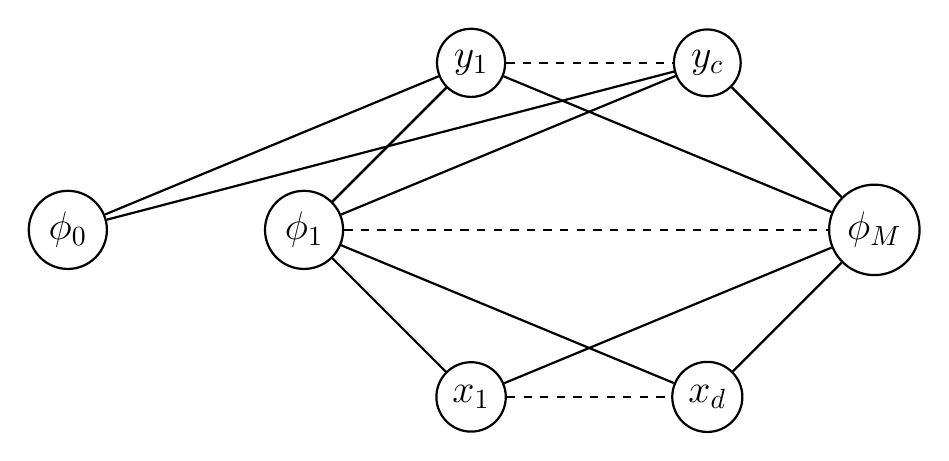
\begin{tikzpicture}[node distance=3cm,
                        thick, 
                        main node/.style={circle, draw, font=\sffamily\Large\bfseries}]
                        
      
      \node[main node] (1) {$y_{1}$};
      \node[main node] (2) [right of=1] {$y_{c}$};
      \node[main node] (3) [below left of=1] {$\phi_{1}$};
      \node[main node] (4) [below right of=2] {$\phi_{M}$};
      \node[main node] (5) [below right of=3] {$x_{1}$};
      \node[main node] (6) [below left of=4] {$x_{d}$};
      \node[main node] (7) [left of=3] {$\phi_{0}$};
      
      
      \draw[thick, dashed] (1) -- (2);
      \draw[thick, dashed] (3) -- (4);
      \draw[thick, dashed] (5) -- (6);
      \draw[thick] (1) -- (3);
      \draw[thick] (1) -- (4);
      \draw[thick] (2) -- (4);
      \draw[thick] (7) -- (1);
      \draw[thick] (7) -- (2);
      \draw[thick] (3) -- (1);
      \draw[thick] (3) -- (2);
      \draw[thick] (3) -- (6);
      \draw[thick] (3) -- (5);
      \draw[thick] (4) -- (5);
      \draw[thick] (4) -- (6);

    \end{tikzpicture}
    \caption{RBF-NN Architecture}
    \label{fig:your_label}
\end{figure}

\subsection{Methodology}

The RBF-NN was utilised for both short-term and long-term 
predictions. For short-term forecasting, 
the model was tested over a 5-month horizon, based on the optimum lag calculated earlier, while the long-term predictions spanned 57 months. 
The data was differenced based on the recommendations of the 
unit root tests conducted earlier to achieve stationarity. 

First, the data was normalised using a z-score normalisation. This is because
neural networks work best with data
that is between a specified range; it ensures that the data is roughly uniformly
distributed between the network inputs and outputs 
(Mendelsohn, 1993, Preprocessing Data for Neural Networks). Following this 
it was necessary to program the RBF-NN into Python. As no specific RBF package exists
in Python, the kernel regression approach outlined by 
\citeboth{bishop1995}, using the GaussianProcessRegressor (GPR) package in Python.

\subsubsection{The Gaussian Process Regressor}

The Scikit GaussianProcessRegressor is based on the 
standard linear regression 
model, equipped with Gaussian noise,

\begin{align} 
    f(x) = x^{T}w, \quad{y = f(x) + \varepsilon}
\end{align}

where $y$ differs from the function values $f(x)$ by noise which is assumed
to follow an independent and identically distributed Gaussian distribution
$\mathcal{N}_1$
\begin{align*}
    \varepsilon \sim \mathcal{N}_1 \bigl(0, \sigma_{n}^2\bigr)
\end{align*}
This assumption together with the model produces the 
probability density of the observations given the inputs, 
which is factored over cases in the training set, 
permissible because of the independence assumption,

\begin{align}
    p(y|X,w) = \prod_{i=1}^{n} p(y_i|x_i ,w) = \mathcal{N}\bigl(X^T, \sigma_{n}^2 I\bigr)
\end{align}

As this is a Bayesian model a \textit{prior distribution} over the parameters must be specified, 
expressing our beliefs about the prior
parameters before the observations are used. A covariance function or kernel
is specified according to the characteristics of the data; in our model this 
is the generalised inverse multiquadric

$$ k(x,x') = \biggl( ||x-x'|| + \sigma^2\biggr)^{-\beta} $$
and used to construct the covariance matrix $K$, which along with 
a mean of $0$ forms the distribution of the the weights 
$$ w \sim \mathcal{N}\bigl(0, K\bigr)$$
By Bayes' Theorem, 

\begin{align}
    p(w|y, X) = \frac{p(y|X,w) p(w)}{p(y|X)}
\end{align}
Using this, the posterior distribution is then obtained

\begin{align}
    p(w|y, X) \sim \mathcal{N}\bigl(\frac{A^{-1}Xy}{\sigma_{n}^{2}}, A^{-1}\bigr) \label{eq:nine}
\end{align}
where the covariance matrix $A^{-1} = K^{-1} + \frac{XX^T}{\sigma_{n}^2}$.
To make predictions on a test case all possible $w$
values, weighted by their posterior probability, are averaged to obtain the
predictive distribution, upon which predicted outputs are computed. \citep{rasmussen2006}

\subsubsection{The Network}

A $4$-dimensional input space $X$
passes inputs $\boldsymbol{\mathrm{x}}_1, \boldsymbol{\mathrm{x}}_2,\ldots \boldsymbol{\mathrm{x}}_{n}$
and corresponding outputs \( y = \{y_1, y_2, \dots, y_n\} \), through the first
layer, in which the covariance function $(x,x')$
is applied, the goal being to determine the distribution of the weights. Prior to this,
the optimal hyperparameters in the covariance function, which plays an analogous
role to the RBF basis function, are calculated using GridSearch Cross Validation; these hyperparameters are:
\begin{enumerate}
    \item $\alpha$: a regularisation parameter which represents a small quantity
    that is added to the diagonals of the covariance matrix to ensure it is 
    invertible. 
    \item $\beta$: the power in the covariance function, which controls the shape of the function.
    \item $\sigma$: a parameter which controls how much of the noise in the data the kernel accounts for; naturally, 
    it moderates the risk of overfitting and underfitting.
    \item Length scale: a parameter that controls the influence - analogous to 
    the width each RBF neuron possesses - that each kernel (analogous to node) is to have.
\end{enumerate}
following this the model uses the training observation $(y,X)$ to find
the posterior predictive distribution, and with it the predicted output, after 
averaging over all possible $w$, weighted by their likelihood according to \eqref{eq:nine}. 

\subsection{Results}

The model returned a mean absolute error of MAE $=0.16$ and 
$R^2 = 9\%$ for the long-term prediction, outperforming the ARDL-ECM model by 
$2.4\%$.


\begin{figure}[h]
    \centering
    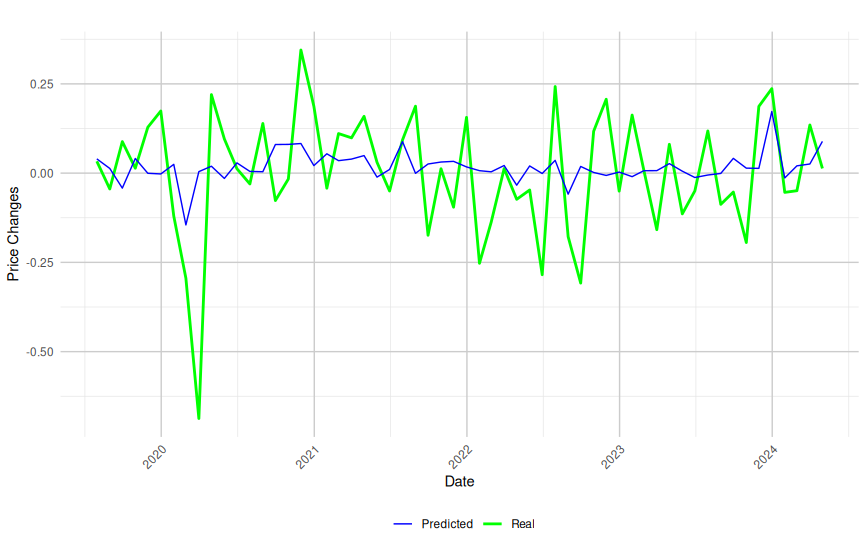
\includegraphics[width=0.8\textwidth]{long-term-monthly.png}
    \caption{Long-term predicted vs monthly real FTSE250 price changes}
    \label{fig:lmonthly}
\end{figure}

The interpretation of this is that, over the long-run (4-5 years), the variations in the 
Consumer Price Index, interest rate, USD/GBP exchange rate, and M3 money 
supply explain or account for $9\%$ of the fluctuations of the
monthly FTSE250 value. This relates closely to the findings of \citeboth{conover1999}, 
who used an econometric model to establish that $4\%$ of the variation in monthly UK stock returns can be 
explained by variations in the money supply. It also suggests a higher level of influence 
than the ARDL-ECM model provided, that only $R^2=3.4\%$ of the monthly FTSE250 variations 
are affected by the selected macroeconomic variables, demonstrating the ability of machine learning
methods to capture patterns in the data unavailable to econometric models. 

\begin{figure}[h]
    \centering
    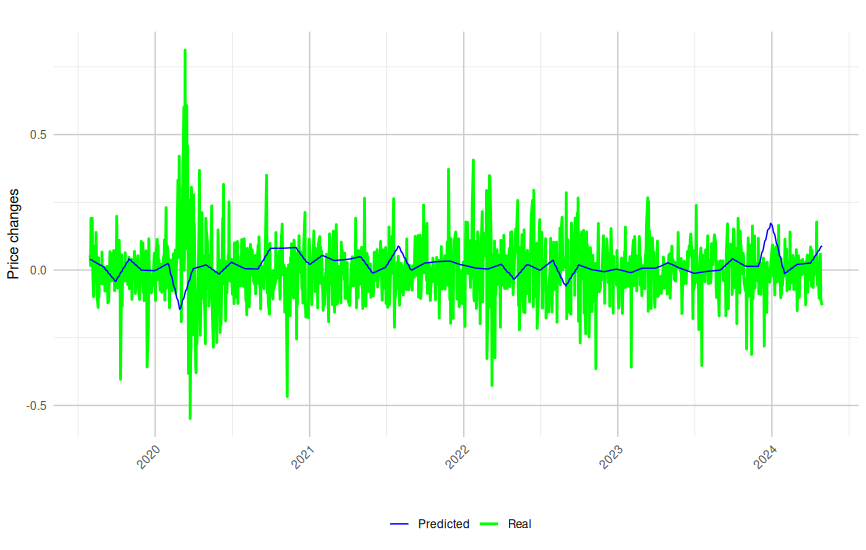
\includegraphics[width=0.8\textwidth]{long-term-daily.png}
    \caption{Long-term predicted vs daily real FTSE250 price changes}
    \label{fig:ldaily}
\end{figure}

In the context of a phenomenon as complex as the stock market,
which is influenced by an inumerable quantity of factors such as investor sentiment
- inherently irrational, 
political instability, geopolitical shocks, corporate governance, and financial regulation, this result 
unsurprising. Furthermore, the selection of economic variables in this study
is by no means exhaustive; commodity prices, international trade dynamics,
economic growth, and many other variables also exert a non-insignificant 
effect on the stock market.

\begin{figure}[h]
    \centering
    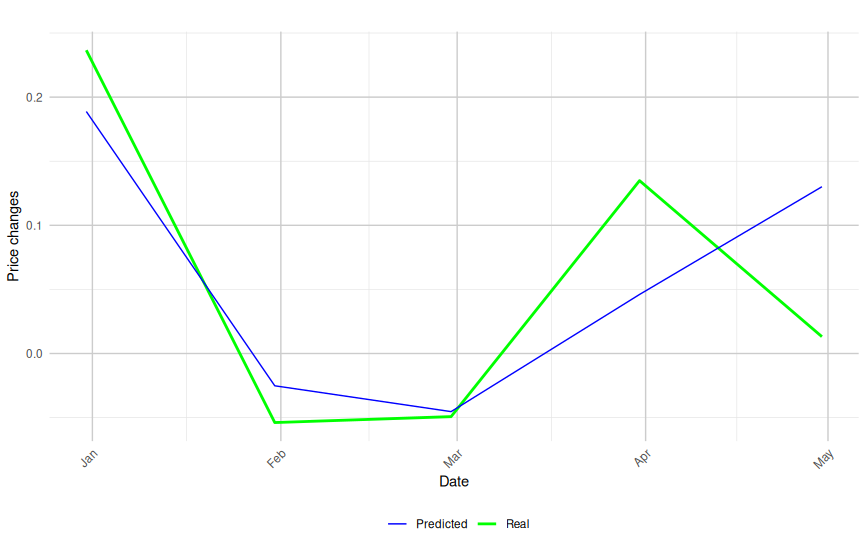
\includegraphics[width=0.8\textwidth]{short-term-monthly.png}
    \caption{Short-term predicted vs monthly real FTSE250 price changes}
    \label{fig:smonthly}
\end{figure}

The short-term prediction yielded MAE = $0.07$ and 
$R^2 = 61\%$, for a 5-month time horizon.
The significantly better performance of the model in the short-run
indicates that the selected macroeconomic variables possesses
a stronger predictive power over shorter periods. This was highlighted 
earlier in the ARDL model, with the interest rate and money supply significantly
impacting the FTSE250 price in the short-run. 

\begin{figure}[h]
    \centering
    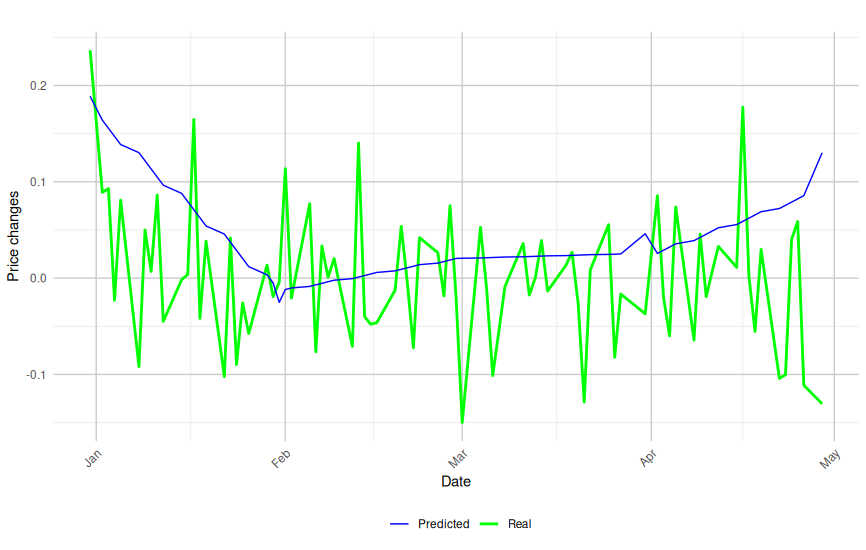
\includegraphics[width=0.8\textwidth]{short-term-daily.png}
    \caption{Short-term predicted vs daily real FTSE250 price changes}
    \label{fig:sdaily}
\end{figure}


In the short-term, which defined as 5 months, 
as per the optimum lag for the FTSE250 in the ARDL model, the market movements
are more closely tied to recent deviations in the economy, because theoretically
the short-run is not exposed to the various unforeseen external shocks and structural changes
that dilute the relationship between these variables and the stock market in the 
long-run. Essentially, as the prediction window expands, 
more uncertainty and unknowns are introduced, which translates into 
lower predictive quality. Furthermore, as the time horizon extends into the long-run, fundamental factors 
begin to matter a lot more. The compound effect of earnings, cash flows and
managerial efficiencies begins to outweigh the 
influence of fluctuating macroeconomic sentiment. Thus, in the short-run 
a different phenomenon is observed.





\section{Conclusion}

This study first tested the findings of previous econometric research on the 
UK stock market, relating the impact of some especially
relevant macroeconomic factors on the FTSE250. 

Stock markets provide important information on the economy, 
and economic policymakers are vigilant in tracking the fluctuations 
in these markets, and try to forecast the 
forthcoming fluctuations based on policy changes that affect the macroeconomy.
Within this context, the study examined the 
impacts of the interest rate, USD/GBP
exchange rate, the consumer price index, and 
M3 money supply market activity on
the FTSE250 index over the October 1993 – April 2024 period.
The results suggest a cointegrated long-run
relationship between the macroeconomic variables and the stock market index. 
The long-run coefficients imply that
increases in the interest rate and depreciation in the exchange rate
significantly depress the FTSE250 value. 
Policymakers dealing with forecasting the UK stock markets
should consider the factors in the study, and to raise the stock
market's value, a lower interest rate regime should be adopted and 
the Pound should be made more competitive.

The the study also investigated the efficacy of machine learning methods in 
the field of stock-econometric forecasting. The RBF-NN performed well in
short-term forecasting of the FTSE250, and offers investors with an accurate forecasting tool, 
to leverage in their trading strategies. The long-term forecast was able to improve on the ARDL-ECM model, and provides 
economists with a tool to compute non-econometric, quantitative measures of the 
long-term influence of macroeconomic variables on the stock market. 

Further research should endeavour to include other macroeconomic variables such as 
foreign direct and portfolio investment, commodity prices and economic growth.
Falling outside the immediate scope of the current study, 
an autoregresive model could also be tried, including the past values of the 
FTSE250 in the input space to provide a more accurate model. In addition, 
a more granular data set could be utilised by applying a 
Brownian bridge algorithm to generate daily macroeconomic data and 
subsequently testing the RBF-NN against other neural networks 
such as auto-regressive LSTMs, as well as other machine learning methods suited for 
forecasting such as Support Vector Machines (SVM). 

\bibliographystyle{plainnat}
\bibliography{paper}

\end{document}
